\chapter{Implementasi dan Pengujian}
\label{chap:Implementasi dan Pengujian}

Pada bab ini akan berisi mengenai implementasi perangkat lunak dan pengujian perangkat lunak yang dibangun.

\section{Implementasi Perangkat Lunak}

Pada bagian ini akan dibahas mengenai tampilan antarmuka perangkat lunak yang sudah dibangun.

\subsection{Tampilan Antarmuka Perangkat Lunak}

Tampilan antarmuka awal perangkat lunak dapat dilihat pada Gambar \ref{fig:tampilan1} dengan keterangan bagian-bagian sebagai berikut.

\begin{itemize}
	\item Bagian no 1 merupakan tombol untuk mengembalikan \textit{password}.
	\item Bagian no 2 merupakan tombol untuk menyimpan \textit{password}.
\end{itemize}

%diagram
\begin{figure}[H]
	\centerline{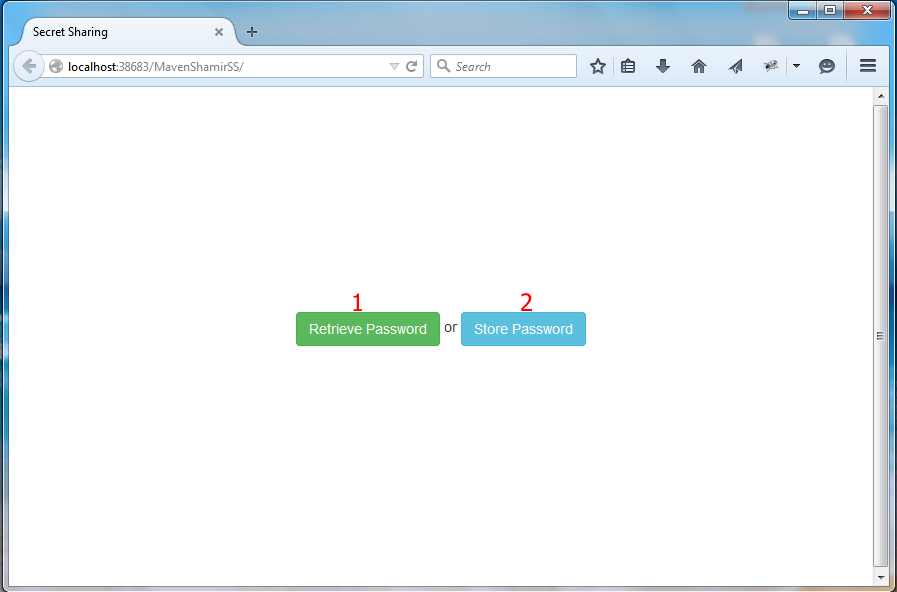
\includegraphics[scale=0.5]{Gambar/tampilan1}}
	\caption{Tampilan antarmuka awal}\label{fig:tampilan1}
\end{figure}

Setelah tombol \textit{"Store Password"} ditekan, tampilan antarmuka perangkat lunak akan terlihat seperti pada Gambar \ref{fig:tampilan2} dengan keterangan sebagai berikut.

\begin{itemize}
	\item Bagian no 3 merupakan tombol untuk menambah \textit{password}. Pengguna minimal harus menambahkan 1 \textit{password}, jika tidak maka akan muncul notifikasi seperti pada Gambar \ref{fig:tampilan2_2}.
	\item Bagian no 4 merupakan tombol untuk menambah pertanyaan keamanan. Pengguna minimal harus menambahkan 5 pertanyaan keamanan, jika kurang maka akan muncul notifikasi seperti pada Gambar \ref{fig:tampilan2_3}.
	\item Bagian no 5 merupakan tombol untuk melanjutkan menyimpan \textit{password}.
	\item Bagian no 6 merupakan tombol untuk kembali ke tampilan antarmuka awal.
	\item Bagian no 7 merupakan teks masukkan untuk pertanyaan keamanan yang hendak ditambahkan.
\end{itemize}

%diagram
\begin{figure}[H]
	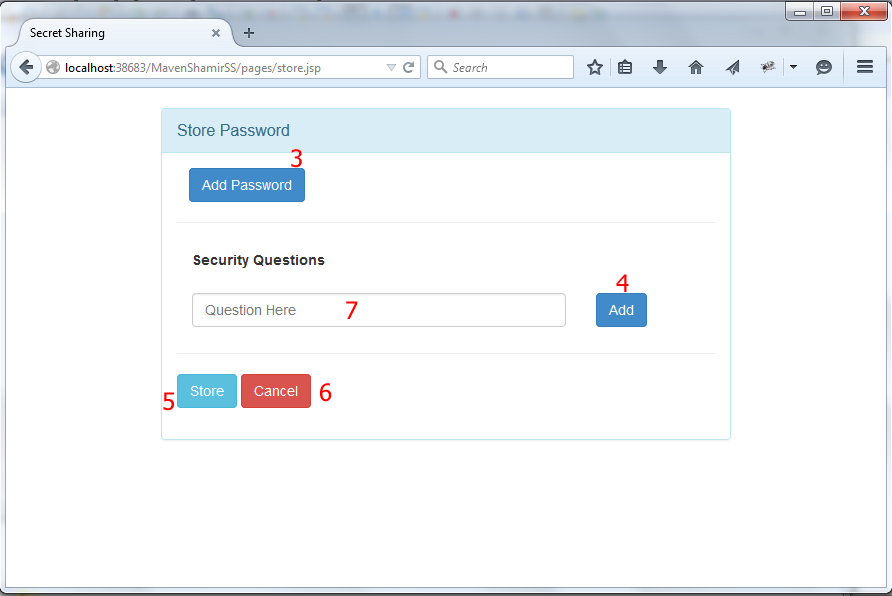
\includegraphics[scale=0.5]{Gambar/tampilan2}
	\centering
	\caption{Tampilan antarmuka untuk menyimpan \textit{password}}\label{fig:tampilan2}
\end{figure}

%diagram
\begin{figure}[H]
	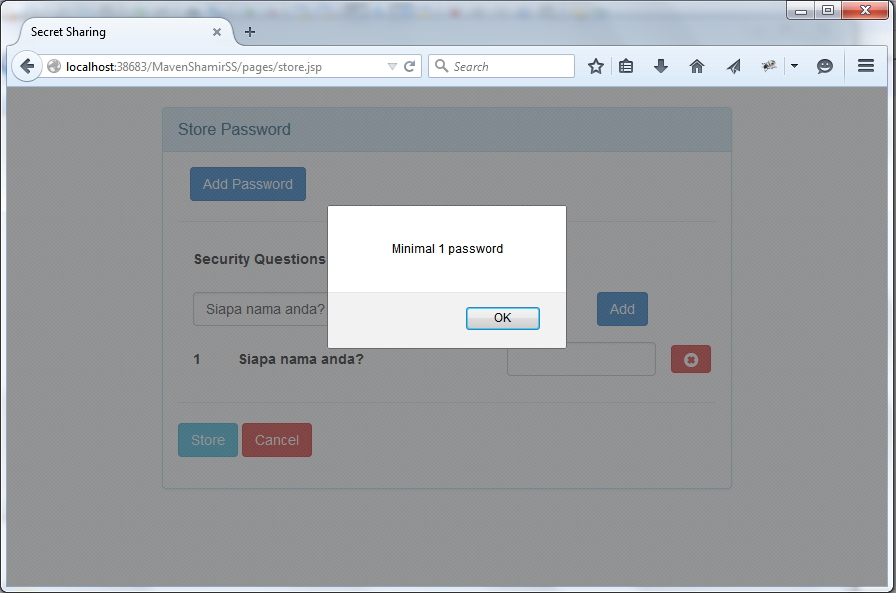
\includegraphics[scale=0.5]{Gambar/tampilan2_2}
	\centering
	\caption{Tampilan antarmuka untuk menyimpan \textit{password}}\label{fig:tampilan2_2}
\end{figure}

%diagram
\begin{figure}[H]
	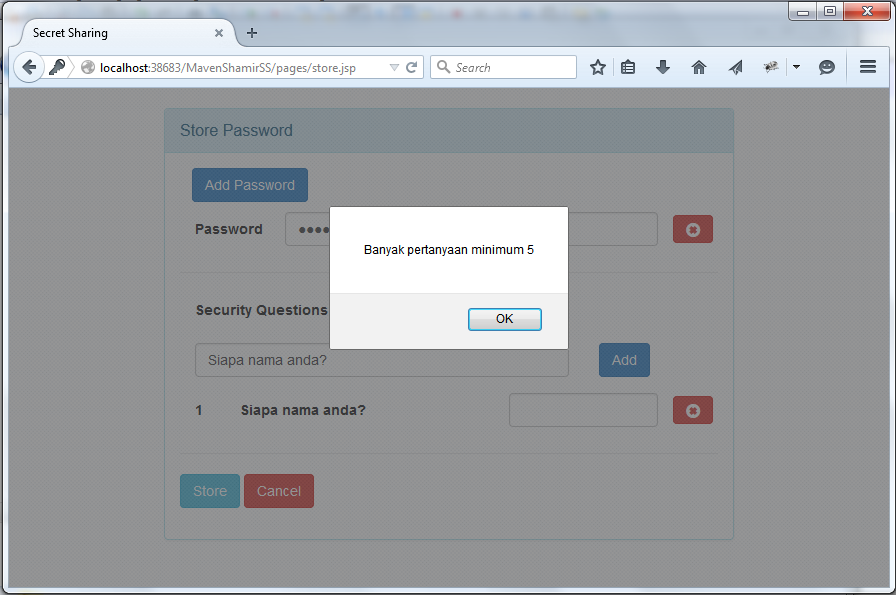
\includegraphics[scale=0.5]{Gambar/tampilan2_3}
	\centering
	\caption{Tampilan antarmuka untuk menyimpan \textit{password}}\label{fig:tampilan2_3}
\end{figure}

Setelah tombol \textit{"Add Password"} ditekan, maka tampilan antarmuka akan menambahkan masukkan teks untuk memasukkan \textit{password} yang hendak disimpan. Setelah tombol \textit{"Add"} ditekan, maka tampilan antarmuka akan menambahkan teks masukkan untuk jawaban dari pertanyaan keamanan yang sudah diisi di Bagian no 7. Tampilan yang ditunjukkan perangkat lunak dapat dilihat pada Gambar \ref{fig:tampilan2_1}.

%diagram
\begin{figure}[H]
	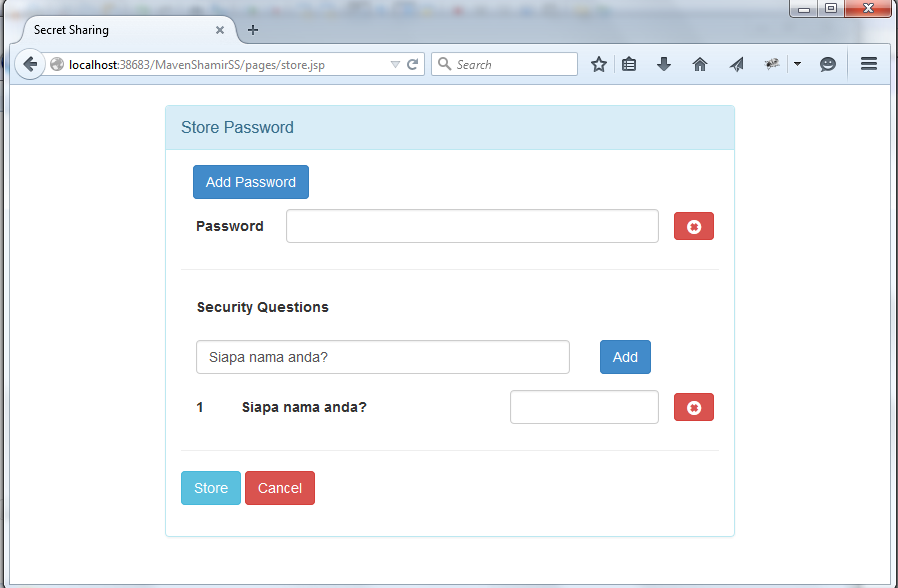
\includegraphics[scale=0.5]{Gambar/tampilan2_1}
	\centering
	\caption{Tampilan antarmuka untuk menyimpan \textit{password}}\label{fig:tampilan2_1}
\end{figure}

Setelah tombol \textit{"Store"} ditekan, maka tampilan antarmuka perangkat lunak akan kembali ke tampilan antarmuka awal. \textit{Password} sudah berhasil disimpan. Kemudian, setelah tombol \textit{"Retrieve Password"} ditekan, maka tampilan perangkat lunak akan terlihat seperti pada Gambar \ref{fig:tampilan3} dengan keterangan sebagai berikut.

\begin{itemize}
	\item Bagian no 8 merupakan bagian dari pertanyaan keamanan yang harus dijawab oleh pengguna.
	\item Bagian no 9 merupakan bagian dari jawaban setiap pertanyaan keamanan yang harus dijawab.
	\item Bagian no 10 merupakan tombol untuk mengembalikan \textit{password}.
	\item Bagian no 11 merupakan tombol untuk kembali ke tampilan antarmuka awal.
\end{itemize}

%diagram
\begin{figure}[H]
	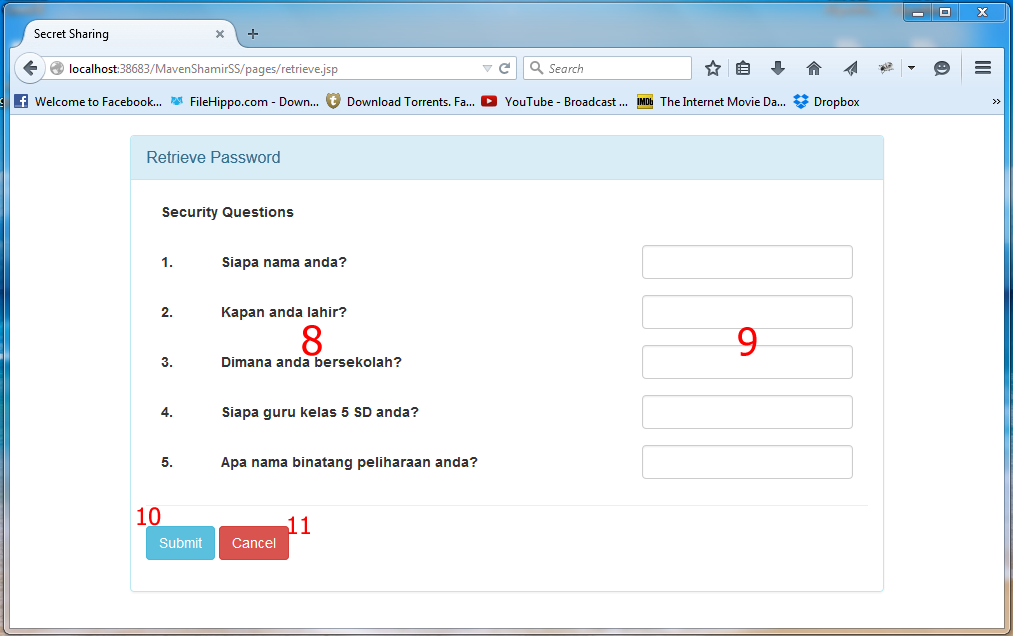
\includegraphics[scale=0.5]{Gambar/tampilan3}
	\centering
	\caption{Tampilan antarmuka untuk mengembalikan \textit{password}}\label{fig:tampilan3}
\end{figure}

Setelah tombol "Submit" pada Gambar \ref{fig:tampilan3} ditekan, perangkat lunak akan memroses setiap pertanyaan dan jawaban. Jika banyak jawaban benar dari pertanyaan keamanan yang dijawab oleh pengguna sesuai dengan minimal banyak pertanyaan keamanan yang dijawab benar yang sudah ditentukan sebelumnya, maka tampilan perangkat lunak akan terlihat seperti pada Gambar \ref{fig:tampilan4}.

%diagram
\begin{figure}[H]
	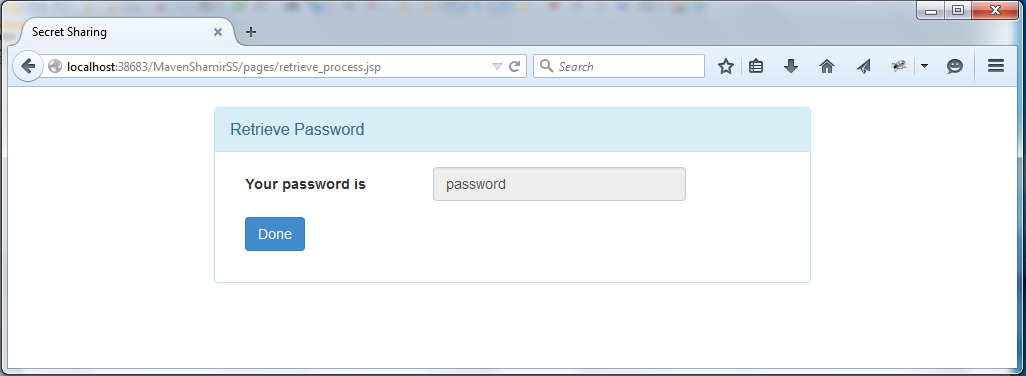
\includegraphics[scale=0.5]{Gambar/tampilan4}
	\centering
	\caption{Tampilan antarmuka untuk mengembalikan \textit{password}}\label{fig:tampilan4}
\end{figure}

Sedangkan, jika tidak sesuai, maka tampilan perangkat lunak akan terlihat seperti pada Gambar \ref{fig:tampilan4_1}.

%diagram
\begin{figure}[H]
	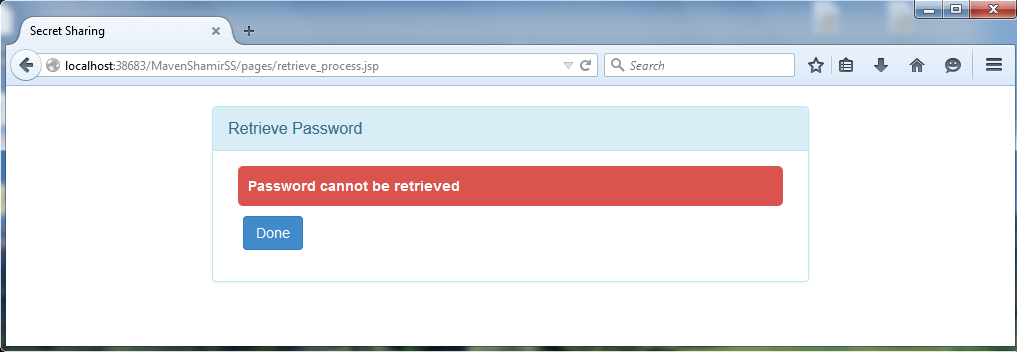
\includegraphics[scale=0.5]{Gambar/tampilan4_1}
	\centering
	\caption{Tampilan antarmuka untuk mengembalikan \textit{password}}\label{fig:tampilan4_1}
\end{figure}

\section{Pengujian Perangkat Lunak}

Pada bagian ini akan berisi tentang metode pengujian, hasil pengujian, analisis pengujian, dan kesimpulan dari pengujian perangkat lunak yang sudah dibangun.

\subsection{Metode Pengujian}

Pengujian terhadap perangkat lunak yang sudah dibangun akan dibagi menjadi 2 bagian, yaitu
\begin{itemize}
	\item Pengujian fungsional
	\item Pengujian survei
\end{itemize}
Pengujian fungsional bertujuan untuk menguji apakah perangkat lunak yang dibangun sudah bisa mengimplementasikan \textit{secret sharing} shamir. Pengujian survei bertujuan untuk menguji bagaimana kualitas pertanyaan keamanan yang dibuat.

\subsection{Hasil Pengujian Fungsional}\label{subsec:hasil_pengujian_fungsional}

Pengujian fungsional adalah pengujian yang dilakukan terhadap perangkat lunak yang sudah dibangun dengan tujuan untuk memastikan bahwa perangkat lunak yang dibangun sudah bisa mengimplementasikan \textit{secret sharing} shamir. Pada bagian ini akan diberikan satu contoh kasus dimana \textit{password} dapat dikembalikan dan satu contoh kasus dimana \textit{password} tidak bisa dikembalikan.

Pada bagian ini juga akan dijelaskan langkah-langkah dimulai dari menyimpan \textit{password} sampai dengan mengembalikan \textit{password}. Dalam contoh kasus untuk pengujian fungsional, banyak \textit{share} 5, \begin{math}n=5\end{math} dan minimal \textit{share} yang dimiliki supaya bisa mengembalikan password sebanyak 4, \begin{math}k=4\end{math}. Langkah awal adalah menyimpan \textit{password}. Gambar \ref{fig:simpan_password} menunjukkan tampilan antarmuka perangkat lunak untuk langkah awal.

%diagram
\begin{figure}[H]
	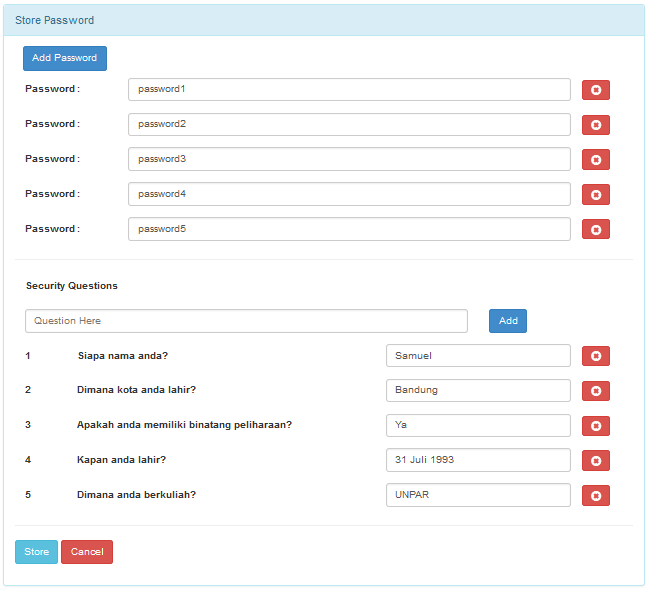
\includegraphics[scale=0.5]{Gambar/simpan_password}
	\centering
	\caption{Langkah menyimpan \textit{password}}\label{fig:simpan_password}
\end{figure}

Pada bagian ini, jenis pertanyaan yang dibuat tidak dipermasalahkan karena tujuannya hanya untuk fungsionalitas. Selain itu, pada bagian masukkan teks untuk \textit{password}, \textit{password} ditunjukkan sekedar bagian dari pengujian. Langkah selanjutnya setelah menyimpan \textit{password} adalah mengembalikan \textit{password}. Gambar \ref{fig:balik_password_sukses} menunjukkan tampilan antarmuka perangkat lunak untuk mengembalikan \textit{password}.

%diagram
\begin{figure}[H]
	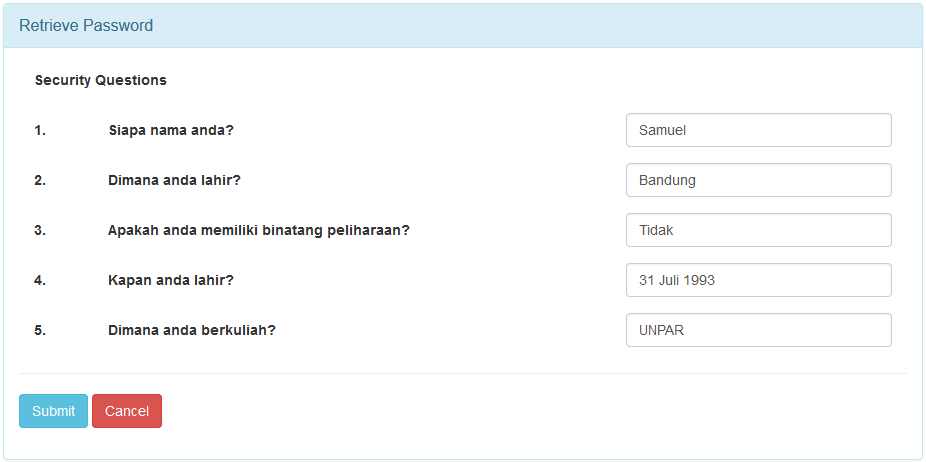
\includegraphics[scale=0.5]{Gambar/balik_password_sukses}
	\centering
	\caption{Langkah menjawab pertanyaan keamanan}\label{fig:balik_password_sukses}
\end{figure}

Gambar \ref{fig:balik_password_sukses} menunjukkan bahwa seluruh pertanyaan keamanan dijawab dengan benar dan \textit{password} akan berhasil dikembalikan. Gambar \ref{fig:balik_password_sukses_next} menunjukkan bahwa \textit{password} berhasil dikembalikan.

%diagram
\begin{figure}[H]
	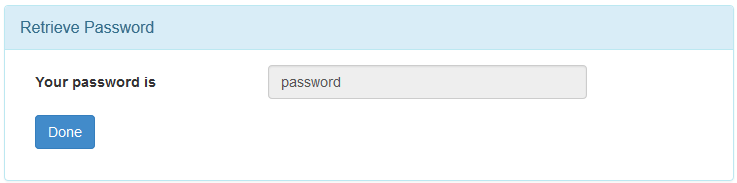
\includegraphics[scale=0.5]{Gambar/balik_password_sukses_next}
	\centering
	\caption{\textit{Password} berhasil dikembalikan}\label{fig:balik_password_sukses_next}
\end{figure}

Contoh kasus diatas adalah contoh kasus \textit{password} berhasil didapatkan, berikutnya akan ditunjukkan contoh kasus dimana \textit{password} tidak berhasil dikembalikan. Langkah awal dimulai langsung dari langkah mengembalikan \textit{password} dan ditunjukkan pada Gambar \ref{fig:balik_password_gagal}.

%diagram
\begin{figure}[H]
	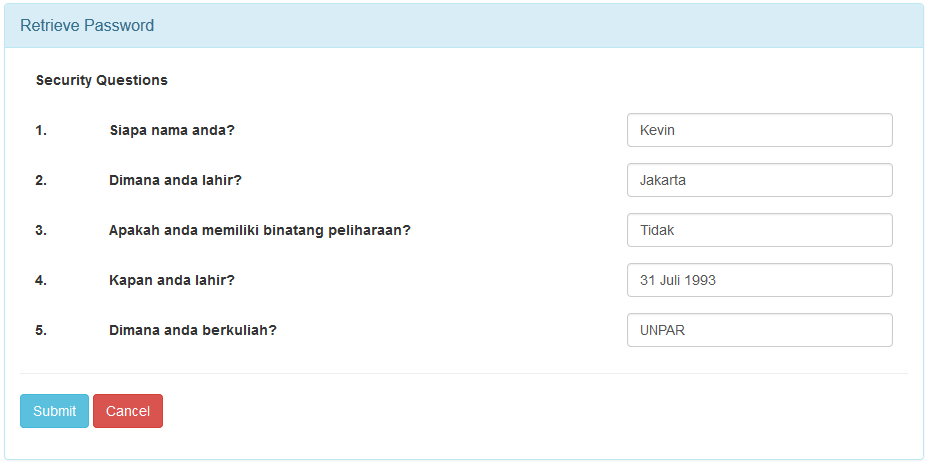
\includegraphics[scale=0.5]{Gambar/balik_password_gagal}
	\centering
	\caption{Langkah menjawab pertanyaan keamanan}\label{fig:balik_password_gagal}
\end{figure}

Gambar \ref{fig:balik_password_gagal} menunjukkan bahwa dari \begin{math}k=4\end{math}, banyak pertanyaan keamanan yang bisa dijawab benar hanya 3 pertanyaan saja atau \begin{math}k-1\end{math}, yaitu pertanyaan nomor 3, 4, dan 5. Gambar \ref{fig:balik_password_gagal_next} menunjukkan bahwa \textit{password} tidak berhasil didapatkan.

%diagram
\begin{figure}[H]
	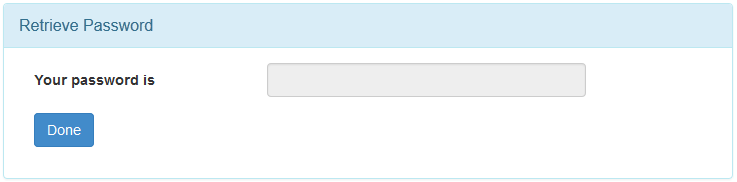
\includegraphics[scale=0.5]{Gambar/balik_password_gagal_next}
	\centering
	\caption{\textit{Password} tidak berhasil dikembalikan}\label{fig:balik_password_gagal_next}
\end{figure}

\subsection{Hasil Pengujian Survei}\label{subsec:hasil_pengujian_survei}

Pada bagian ini akan ditunjukkan hasil pengujian survei. Hasil pengujian survei bertujuan untuk menilai kualitas dari pertanyaan keamanan dengan melihat tingkat kesulitan untuk menebak atau menjawab jawaban benar. Asumsi yang digunakan dalam pengujian ini adalah seluruh jawaban relevan dengan pertanyaan keamanan.

Pengujian survei ini dilakukan terhadap 7 orang responden terbagi atas 4 kasus. Responden melakukan survei dengan cara mencoba untuk menebak jawaban dari pertanyaan keamanan untuk mengembalikan password. Setiap orang bebas memilih cara untuk mendapatkan jawaban dari pertanyaan selain tidak bertanya kepada pembuat pertanyaan keamanan. 

Tujuh orang responden yang melakukan survei terdiri dari 3 responden teman, 2 responden teman dekat, dan 2 responden keluarga dari pembuat pertanyaan keamanan. Kasus yang digunakan untuk pengujian survei terbagi menjadi 4 topik, yaitu
\begin{itemize}
	\item Topik kasus 1: pertanyaan yang kemungkinan jawabannya hanya 2, yaitu Ya dan Tidak dan pertanyaan yang bisa ditemukan dalam sosial media.
	\item Topik kasus 2: pertanyaan yang jawabannya berupa angka (tanggal lahir, bulan, tahun, dan sebagainya) dan pertanyaan yang tidak stabil, yaitu ketika mengisi dan nanti menjawab belum tentu sama.
	\item Topik kasus 3: pertanyaan keamanan yang sifatnya personal (ada kemungkinan bisa dijawab bila ada hubungan keluarga).
	\item Topik kasus 4: gabungan dari topik 1, 2, dan 3 secara merata.
\end{itemize}

Setiap kasus memiliki minimal banyak pertanyaan keamanan yang dijawab benar yang sama, \begin{math}n=10, k=4\end{math}. Berikut tabel hasil survei untuk setiap kasus beserta dengan penjelasannya.

\subsubsection{Kasus 1}

Berikut daftar pertanyaan keamanan yang digunakan dalam kasus 1.
\begin{itemize}
	\item Apa jenis kelamin anda? (Laki-laki/Perempuan)
	\item Apakah anda pernah ke luar negeri?
	\item Apakah anda mempunyai binatang peliharaan?
	\item Apakah anda bermain alat musik?
	\item Apakah anda pernah tidak naik kelas?
	\item Apakah anda pernah mengalami kecelakaan?
	\item Apakah anda menyukai kegiatan olahraga?
	\item Apa nama belakang anda?
	\item Siapa nama ibu anda?
	\item Siapa nama ayah anda?
\end{itemize}
Kemudian, Grafik \ref{fig:kasus1} menunjukkan hasil survei kasus 1.
%diagram
\begin{figure}[H]
	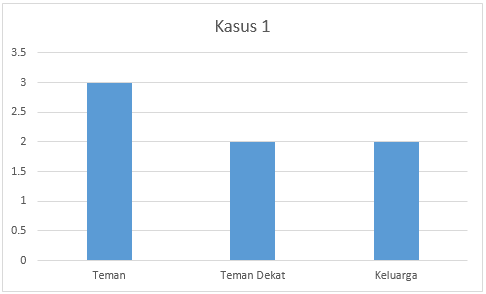
\includegraphics[scale=0.7]{Gambar/kasus1}
	\centering
	\caption{Pengujian survei kasus 1}\label{fig:kasus1}
\end{figure}

\subsubsection{Kasus 2}

Berikut daftar pertanyaan keamanan yang digunakan dalam kasus 2.
\begin{itemize}
	\item Pada tahun berapa anda lahir?
	\item Pada tanggal berapa anda lahir?
	\item Pada bulan apa anda lahir?
	\item Berapa perbedaan umur anda dengan ayah anda?
	\item Berapa perbedaan umur anda dengan ibu anda?
	\item Berapa orang saudara anda?
	\item Berapa nomor rumah tempat anda tinggal?
	\item Dimana anda tinggal?
	\item Apa merek kendaraan yang anda pakai?
	\item Pada hari apa anda lahir?
\end{itemize}

Kemudian, Grafik \ref{fig:kasus2} menunjukkan hasil survei kasus 2.
%diagram
\begin{figure}[H]
	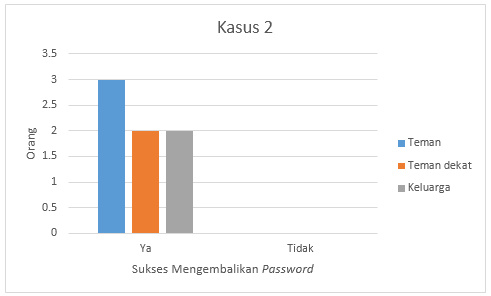
\includegraphics[scale=0.7]{Gambar/kasus2}
	\centering
	\caption{Pengujian survei kasus 1}\label{fig:kasus2}
\end{figure}

\subsubsection{Kasus 3}

Berikut daftar pertanyaan keamanan yang digunakan dalam kasus 3.
\begin{itemize}
	\item Pada jam berapa anda lahir?(jj:mm)
	\item Apa nama sekolah dasar tempat anda bersekolah?
	\item Siapa nama belakang sepupu paling tua dari keluarga sisi ibu anda?
	\item Siapa nama belakang sepupu paling tua dari keluarga sisi ayah anda?
	\item Apa cita-cita anda dulu sewaktu kecil?
	\item Siapa nama anak paling tua dari nenek sisi ibu anda?
	\item Apa binatang peliharaan pertama anda?
	\item Apa alat musik yang anda mainkan pertama kali?
	\item Dimana kerabat terdekat anda tinggal/berasal?
	\item Siapa nama guru kelas 3 SD anda?
\end{itemize}

Tidak ada responden yang berhasil mengembalikan password untuk kasus 3, karena dari itu grafik untuk kasus 3 tidak ditunjukkan.

\subsubsection{Kasus 4}

Untuk kasus 4, karena merupakan gabungan dari kasus 1, 2, dan 3 maka banyak pertanyaan pun ditambah menjadi 15 pertanyaan, masing-masing 5 pertanyaan untuk setiap kasus.

Berikut daftar pertanyaan keamanan yang digunakan dalam kasus 4.
\begin{itemize}
	\item Apakah anda mempunyai binatang peliharaan?
	\item Apakah anda bermain alat musik?
	\item Apakah anda pernah tidak naik kelas?
	\item Apa nama belakang anda?
	\item Siapa nama ibu anda?
	\item Pada hari apa anda lahir?
	\item Pada tanggal berapa anda lahir?
	\item Pada bulan apa anda lahir?
	\item Berapa perbedaan umur anda dengan ayah anda?
	\item Berapa nomor rumah tempat anda tinggal?
	\item Pada jam berapa anda lahir?(jj:mm)
	\item Apa cita-cita anda dulu sewaktu kecil?
	\item Siapa nama anak paling tua dari nenek sisi ibu anda?
	\item Apa binatang peliharaan pertama anda?
	\item Siapa nama guru kelas 3 SD anda?
\end{itemize}

Kemudian, Grafik \ref{fig:kasus4} menunjukkan hasil survei kasus 4.
%diagram
\begin{figure}[H]
	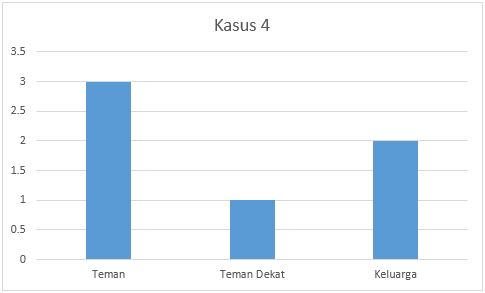
\includegraphics[scale=0.7]{Gambar/kasus4}
	\centering
	\caption{Pengujian survei kasus 1}\label{fig:kasus4}
\end{figure}

\subsection{Analisis Pengujian}

Dari data-data hasil pengujian pada bagian subbab \ref{subsec:hasil_pengujian_fungsional} dan subbab \ref{subsec:hasil_pengujian_survei} akan dilakukan analisis. Untuk data hasil pengujian pada subbab \ref{subsec:hasil_pengujian_fungsional} akan dilakukan analisis mengenai tingkat keberhasilan implementasi \textit{secret sharing} shamir pada perangkat lunak yang dibangun. Untuk data hasil pengujian pada subbab \ref{subsec:hasil_pengujian_survei} akan dilakukan analisis kualitas pertanyaan keamanan yang dibangun serta hubungannya dengan tingkat keberhasilan mengembalikan \textit{password}.

Dinilai dari tingkat keberhasilan implementasi \textit{secret sharing} shamir pada perangkat lunak bisa disebut berhasil. Dalam kasus untuk mengembalikan \textit{password} pada subbab \ref{subsec:hasil_pengujian_fungsional}, dengan menjawab benar 4 pertanyaan atau lebih, \textit{password} bisa dikembalikan, tetapi jika pertanyaan yang dijawab benar kurang 1 atau lebih, dalam kasus ini, kurang dari 4 pertanyaan yang dijawab benar, maka \textit{password} tidak bisa dikembalikan. Hal ini berarti implementasi \textit{secret sharing} shamir pada perangkat lunak bisa dinilai berhasil.

Selanjutnya adalah analisis kualitas pertanyaan keamanan yang dibangun serta efek dan hubungannya dengan tingkat keberhasilan mengembalikan password. Dilihat dari grafik \ref{fig:kasus1} untuk topik kasus 1, karena mayoritas kemungkinan jawaban dari pertanyaan keamanan adalah kemungkinan biner dengan hanya 2 kemungkinan saja (Ya atau Tidak), maka responden bisa dengan mudah mengembalikan \textit{password}.

Dilihat dari grafik \ref{fig:kasus2} untuk topik kasus 2, tingkat keberhasilan untuk mengembalikan password cukup tinggi karena hampir seluruh responden berhasil untuk mengembalikan password. Hal ini disebabkan karena kemungkinan jawaban dari pertanyaan keamanan hanya berupa angka saja, khususnya hanya tanggal ulang tahun, bulan lahir, atau tahun lahir.

Responden dapat menjawab tanggal lahir karena hanya memiliki 30-31 kemungkinan, sedangkan untuk bulan hanya ada 12 kemungkinan, dan juga beberapa pertanyaan lain yang menyangkut angka. Dapat dilihat juga, bahwa beberapa jawaban untuk pertanyaan keamanan merupakan informasi yang sering ditunjukkan dalam profil sosial media, karena dari itu jawaban yang tepat bisa dengan mudah didapatkan.

Untuk topik kasus 3, tidak ada responden yang berhasil mengembalikan \textit{password}. Hal ini karena beberapa pertanyaan sifatnya sangat personal yang bahkan hanya sebagian dari responden keluarga yang mengetahui jawabannya. Pertanyaan yang sifatnya sangat personal akan mempersulit untuk mengembalikan \textit{password} kecuali bagi pembuat pertanyaan.

Dilihat dari grafik \ref{fig:kasus4} untuk topik kasus 4, tingkat keberhasilannya tetap tinggi walaupun topik kasus 4 ini merupakan gabungan dari topik kasus 1, 2, dan 3. Hal ini disebabkan karena mayoritas terdiri pertanyaan dari kasus 1 dan kasus 2 sehingga responden masih bisa mengembalikan \textit{password}.

Responden hanya cukup menjawab 6 pertanyaan benar dari 15 pertanyaan dalam kasus 4, maka responden pun cukup menjawab 3 pertanyaan dari kasus 1 dan 3 pertanyaan dari kasus 2 dengan benar, responden tidak perlu menjawab satupun pertanyaan dari kasus 3. Dapat disimpulkan, bahwa gabungan tidak meningkatkan keamanan dari password untuk bisa dikembalikan hanya oleh pembuat pertanyaan.

\subsection{Kesimpulan Pengujian}

Dari 4 kasus pengujian yang dilakukan maka bisa ditarik beberapa kesimpulan dalam penilaian kualitas pertanyaan keamanan personal. Pertanyaan keamanan personal harus memiliki 5 sifat:
\begin{itemize}
	\item Aman \\
	Pertanyaan keamanan harus tidak mudah ditebak dan tidak mudah diselidiki (\textit{googling}).
	\item Stabil \\
	Pertanyaan keamanan tidak boleh berubah seiring berjalannya waktu.
	\item Mudah diingat \\
	Pertanyaan keamanan harus sifatnya personal sehingga mudah untuk diingat.
	\item Simpel \\
	Pertanyaan keamanan harus sederhana tetapi sifatnya tetap personal.
	\item Memiliki banyak kemungkinan jawaban \\
	Pertanyaan keamanan tidak boleh hanya memiliki kemungkinan jawaban yang sedikit karena akan mudah ditebak (dengan teknik \textit{brute force}).
\end{itemize}

Namun, beberapa pertanyaan keamanan mungkin memiliki banyak kemungkinan jawaban dan aman sehingga tidak mudah ditebak tetapi tidak mudah diingat karena jawabannya terlalu rumit. Beberapa pertanyaan keamanan juga mungkin tidak sesuai dengan situasi atau keadaan dari pembuat pertanyaan. Sehingga, tidak ada pertanyaan keamanan yang memiliki tepat 5 sifat yang diatas.